\documentclass[../main.tex]{subfiles}
\graphicspath{{\subfix{../images/}}}
\begin{document}
\section{Methods and methodology}
\label{methods and methodology}

In this section, we will inspect the methods and methodologies used for the development of this work. In particular, we will give a detailed look at the tools used and why who choose to use them. The section is divided in 3 subsections: "Silero VAD", "WebRTC" and "aiortc". 

\subsection{Silero VAD}

In an article on The Gradient, "One Voice Detector to Rule Them All" \cite{veysov20202onevoice}, Alexander Veysov a Data Scientist in Silero, presents the Silero VAD tool. Silero VAD is a neural voice activity detector that shows great performances and results with the following very important criteria:

\begin{itemize}
    \item High quality
    \item Highly portable
    \item No string attached
    \item Supports 8 and 16 kHz
    \item Supports chunks over 30 ms
    \item Trained on more than 100 languages 
    \item Has good performances in terms of latency
\end{itemize}

The reason why Silero decided to publish their own internal VAD is because it was a problem to find a high quality VAD with a permissible license. Academic solutions are usually slow, not supported and doesn't support streaming. Commercial solutions have typically strings attached in some forms of telemetry and are not "free". Furthermore, Google’s formidable WebRTC VAD is an established and well-known solution, but it has started to show its age. 

Silero VAD uses a multi-head attention (MHA) based neural network with the Short-time Fourier transform as features. "This architecture was chosen due to the fact that MHA-based networks have shown promising results in many applications ranging from natural language processing to computer vision and speech processing" Veysov affirms. 

A multi-head attention neural network is a transformer that uses the multi-head attention technique. The Transformer architecture was quickly established as the leading architecture for most text data applications because it excels at handling text which is inherently sequential. This architecture takes a text sequence as input and produce another text sequence as output. At its core, it contains a stack of Encoder layers and Decoder layers. The Encoder stack and the Decoder stack each have their corresponding Embedding layers for their respective inputs. The Encoder contains the all-important Self-attention layer that computes the relationship between different words in the sequence, as well as a Feed-forward layer. The Decoder contains the Self-attention layer and the Feed-forward layer, as well as a second Encoder-Decoder attention layer, and each Encoder and Decoder has its own set of weights. The Transformer architecture uses self-attention by relating every word in the input sequence to every other word and this enables the model to focus on other words in the input that are closely related to that word. Attention is used in the Transformer in three places: 

\begin{itemize}
    \item Self-attention in the Encoder — the input sequence pays attention to itself
    \item Self-attention in the Decoder — the target sequence pays attention to itself
    \item Encoder-Decoder-attention in the Decoder — the target sequence pays attention to the input sequence
\end{itemize}

In Figure \ref{fig:transformer} it is shown a typical Transformer architecture, highlighting where the attention layers are used.

\begin{figure}[ht]
    \centering
    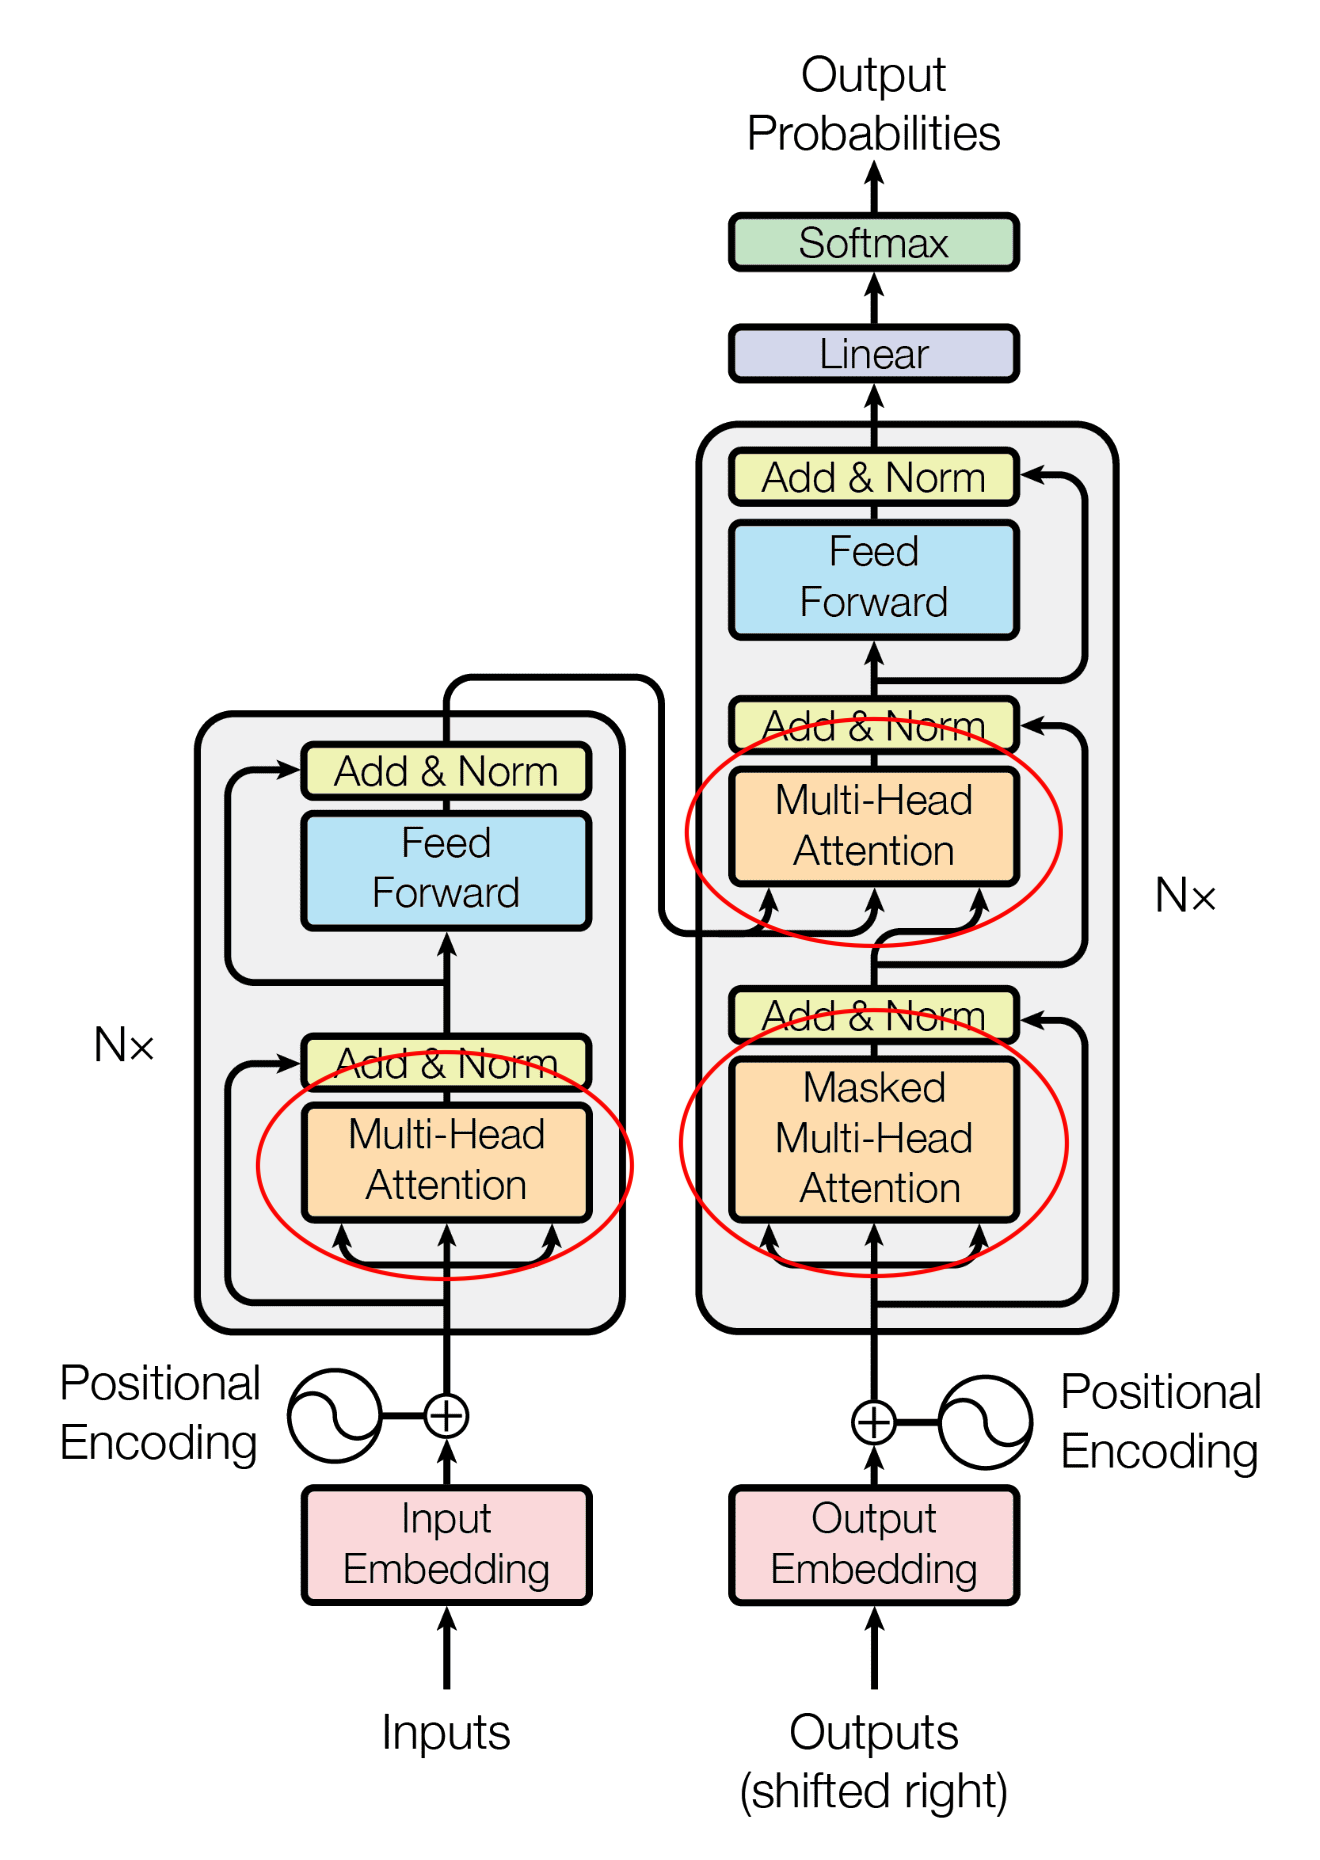
\includegraphics[width=0.7\textwidth]{images/Transformer.png}
    \caption{Transformer architecture highlighting where the attention is used.}
    \label{fig:transformer}
\end{figure}

The Attention layer takes its input in the form of three parameters, known as the Query, Key, and Value. All three parameters are matrices similar in structure, with each word in the sequence represented by a vector. Using multiple attention heads means that the keys, queries, and values input matrices are simply broken up by feature into different heads, each of which are responsible for learning a different representation. For each attention head, the attention mechanism computes a weighted sum of the values for each position in the input sequence. This is similar to the standard self-attention mechanism but is done independently for each head. The attention score between a query element and a key element is computed using a similarity function (often the dot product or a scaled dot product) and is scaled to control the magnitude. And at the end each head is concatenated back together to produce a final Attention score. This creates a single vector for each position in the input sequence but with information from multiple attention heads.

As input to the Silero VAD architecture there isn't a sequence of words, but instead a sequence of features extracted from the audio chunk. In particular the model uses as inputs the Short-time Fourier transform of the signal (STFT). The STFT used as features extracted from the signal enter the category of both formant structure and stationarity analysis described in section \ref{voice activity detection}. 

The Short-Time Fourier Transform (STFT) is a signal processing technique used to analyze how the frequency content of a signal changes over time. It is a common method for analyzing non-stationary signals, which are signals whose characteristics (such as frequency components) change over time. The STFT is a modification of the standard Fourier Transform, which analyzes the frequency components of a signal as if it were stationary. The STFT works by dividing the signal into smaller overlapping segments, often referred to as "windows" or "frames." For each of these segments, a standard Fourier Transform is computed, giving a snapshot of the signal's frequency content for that specific time interval. By applying this process over the entire duration of the signal with these overlapping segments, you can build a time-frequency representation of the signal, showing how its frequency content changes over time. Mathematically, the STFT is defined as follows:

\[ STFT(t, f) = \int_{-\infty}^{\infty} [x(\tau) \cdot w(\tau - t)] \cdot e^{-j2\pi f\tau} \, d\tau \]

The output of the STFT, is a time-frequency representation that reveals how the frequency content of the signal changes over time. By computing the STFT for different time points, we can obtain a spectrogram, which provides a visual representation of the signal's time-varying frequency content. The spectrogram is a widely used tool in audio signal processing, allowing us to analyze and visualize various audio phenomena such as pitch, harmonics, and transient events. For this reason it is vastly used in speech recognition, music analysis, and sound synthesis \cite{stft}.

The Silero VAD model was trained on approximately 13k hours of speech spanning more than 100 languages. Regarding the quality metrics, the model was tested on the Libryparty dataset and the AVA Spoken Activity Datasets, obtaining the ROC-AUC score shown in the table \ref{tab:silero-comparison} below \cite{SileroVAD}. In the table are shown the results of the version 3 and the last version of the model and also the results obtained with other VAD. For the Silero models it is also specified the audio sampling option between 8 and 16 kHz:


\begin{table}[ht]
    \centering
    \begin{tabular}{|l|c|c|} \hline 
         Model&  AVA& LibryParty\\ \hline 
         Silero v4 16k&  0.9& 0.99\\ \hline 
         Silero v4 8k&  0.89& 0.97\\ \hline 
         Silero v3 16k&  0.87& 0.93\\ \hline 
         Silero v3 8k&  0.85& 0.94\\ \hline 
         SpeechBrain&  0.85& 0.99\\ \hline 
         WebRTC&  0.66& 0.81\\ \hline
    \end{tabular}
    \caption{Comparison between ROC-AUC score of different VAD solutions \cite{SileroVAD}}
    \label{tab:silero-comparison}
\end{table}

\newpage

In Figure \ref{fig:precision-recall curve} are shown the precision-recall curve of the Silero VAD model with respect to other solutions. The commercial VAD present in the figure is the PicoVoice VAD.

\begin{figure}[ht]
    \centering
    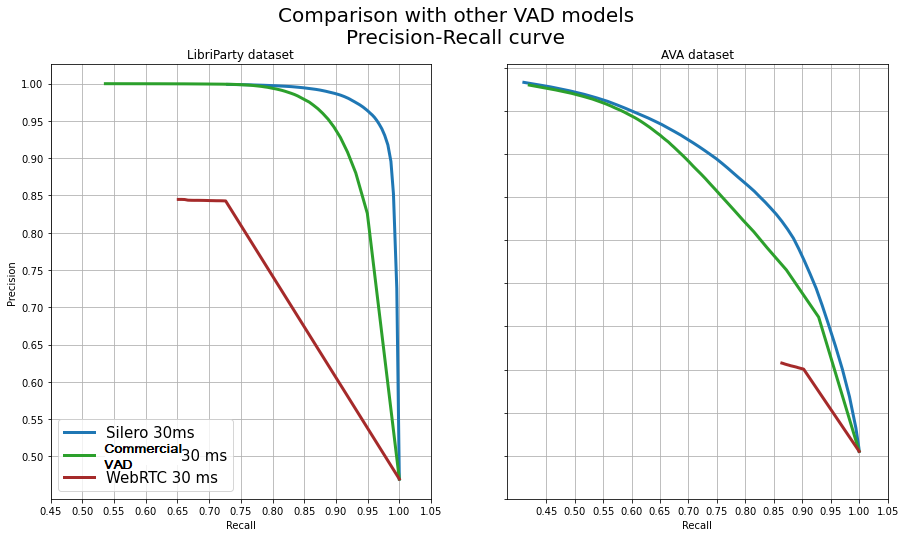
\includegraphics[width=\textwidth]{images/silero-comparison.png}
    \caption{Precision-recall curve comparison with other solutions \cite{SileroVAD}}
    \label{fig:precision-recall curve}
\end{figure}

The following code in listing \ref{listing:silero example} shows a simple example on how the model is used in python with the PyTorch framework. A more detailed utilization for this work is present in section \ref{implementation}.

\begin{lstlisting}[language=Python, caption=Silero Vad usage example]
import torch
torch.set_num_threads(1)

model, utils = torch.hub.load(repo_or_dir='snakers4/silero-vad', model='silero_vad')
(get_speech_timestamps, _, read_audio, _, _) = utils

wav = read_audio('test.wav', sampling_rate=16000)
speech_timestamps = get_speech_timestamps(wav, model, sampling_rate=16000, visualize_probs=True, return_seconds=True)
\end{lstlisting}
\label{listing:silero example}

To conclude we decided to use this voice activity detector for it's ease of use, permissible license and great quality and performance metrics.  

\subsection{WebRTC}
\label{webrtc}

WebRTC (Web Real-Time Communication) is a set of open-source APIs and protocols that enable real-time communication between web browsers and mobile applications. It supports video, voice, and generic data to be sent between peers, allowing developers to build powerful voice and video-communication solutions, without the need for third-party plugins or additional software installations. The technology is available on all modern browsers as well as on native clients for all major platforms and the technologies behind WebRTC are implemented as an open web standard and available as regular JavaScript APIs in all major browsers. The WebRTC project is open-source and supported by Apple, Google, Microsoft and Mozilla, amongst others \cite{WebRTC}.

The WebRTC standard covers, on a high level, two different technologies: media capture devices and peer-to-peer connectivity. Cameras and microphones are commonly referred to as Media Devices and can be accessed with JavaScript through the navigator.mediaDevices object, which implements the MediaDevices interface. 

In particular the getUserMedia() function of the MediaDevices interface returns a MediaStream object that represents a stream of media content, which consists of tracks (MediaStreamTrack) of audio and video. You can retrieve all the tracks from MediaStream by calling MediaStream.getTracks(), which returns an array of MediaStreamTrack objects.

The peer-to-peer connectivity is handled by the RTCPeerConnection interface. This is the central point for establishing and controlling the connection between two peers in WebRTC. RTCPeerConnection needs a mechanism to coordinate communication and to send control messages, a process known as signaling. Unfortunately signaling methods and protocols are not specified by WebRTC and are not part of the API. This means that developers can choose the best signaling method among the messaging protocols they prefer and any two-way communication channel. Signaling is used to exchange three types of information \cite{Get_started_with_WebRTC}:

\begin{itemize}
    \item Session control messages: to initialize or close communication and report errors.
    \item Network configuration: to the outside world, what's your computer's IP address and port?
    \item Media capabilities: what codecs and resolutions can be handled by your browser and the browser it wants to communicate with?
\end{itemize}

The exchange of information through signaling must have completed successfully before peer-to-peer streaming can begin. Once the RTCPeerConnection is created we need to create an SDP offer or answer, depending on if we are the calling peer or receiving peer. To initiate the peer connection setup from the calling side, we create a RTCPeerConnection object and then call createOffer() to create a RTCSessionDescription object. This session description is set as the local description using setLocalDescription() and is then sent over our signaling channel to the receiving side. On the receiving side, we wait for an incoming offer before we create our RTCPeerConnection instance. Once that is done we set the received offer using setRemoteDescription(). Next, we call createAnswer() to create an answer to the received offer. This answer is set as the local description using setLocalDescription() and then sent to the calling side over our signaling server. In the end the calling side must set the receiving's side answer as a remote session description with the setRemoteDesctiption() function. The offer/answer architecture previously described is called JavaScript Session Establishment Protocol, or JSEP. 

After sending metadata information, in order to exchange actual data, WebRTC peers needs to exchange also connectivity information. This is because RTCPeerConnection attempts to connect clients directly or peer-to-peer. In a simpler world, every WebRTC endpoint would have a unique address that it could exchange with other peers in order to communicate directly. In reality, most devices live behind one or more layers of NAT, some have antivirus software that blocks certain ports and protocols, and many are behind proxies and corporate firewalls. In order for the WebRTC clients to communicate behind NAT, WebRTC uses the Interactive Connectivity Establishment (ICE) framework as a technique for NAT traversal. ICE works by exchanging a multiplicity of IP addresses and ports, which are then tested for connectivity by peer-to-peer connectivity checks. The idea is to find the best path to connect peers. ICE first tries to make a connection using the host address obtained from a device's operating system and network card. If that fails (which it will for devices behind NATs), ICE obtains an external address using a STUN server and, if that fails, traffic is routed through a TURN relay server. In other words, a STUN server is used to get an external network address and TURN servers are used to relay traffic if direct (peer-to-peer) connection fails \cite{STUN_TURN}. It is possible to specify STUN and TURN servers in the iceServers configuration object passed to the RTCPeerConnection constructor. 

The Figure \ref{fig:webrtc architecture} shows the WebRTC software architecture, and it shows how this Web API hides a lot of complexities to the developer. 

\begin{figure}[ht]
    \centering
    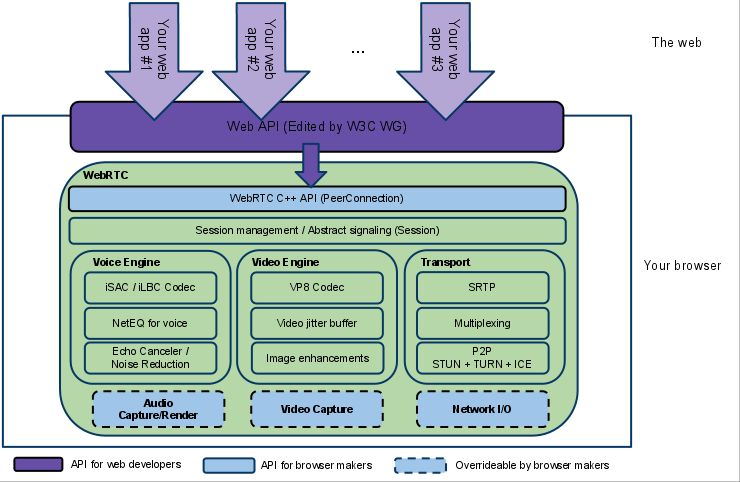
\includegraphics[width=\textwidth]{images/WebRTC architecture.png}
    \caption{WebRTC architecture \cite{WebRTC_architecture}}
    \label{fig:webrtc architecture}
\end{figure}

We decided to use WebRTC for this work because of its ease of use. In particular, it handles otherwise very complicated communication details in a very simple manner. Furthermore, it offers amongst the best real time communication performances and this is why it is also used in very important real time communication applications as Google Meet, Facebook Messenger and Discord.

\subsection{aiortc}

aiortc is a library for Web Real-Time Communication (WebRTC) and Object Real-Time Communication (ORTC) in Python. It is built on top of asyncio, Python's standard asynchronous I/O framework \cite{aiortc}.

The reason for the need of this library is that the WebRTC and ORTC implementations are built into web browsers and do not provide Python bindings. Furthermore, they use an internal Media Stack making hard to use the media inside the stack for audio or video processing. In contrast, the aiortc implementation is quite easy and let to use to media received with the WebRTC APIs in a quite easy way. This thanks to the Media Helpers that are not part of the WebRTC or ORTC APIs, but provide high-level helpers for manipulating media streams.  

Regarding the WebRTC connection and streaming part the library closely follows the Javascript counterpart with the presence of all the main classes like RTCPeerConnection and MediaStreamTrack. It's important to notice that the library in contrast with the Javascript API misses all the APIs the manage the devices, for example the MediaDevices interface with the very useful getUserMedia() function. This means that getting the video or audio source of the stream is in charge of the developer. 

As said before, for the handling of the media streams, the library provides some high-level helpers that are divided into: Media sources, Media sinks and Media transforms. The Media sources provides a MediaPlayer object that is a way to read audio and video sources from a file or a webcam. These sources return a MediaStreamTrack object that can be sent to the remote peer with the RTCPeerConnection class. The Media sinks are the MediaRecorder and the MediaBlackhole. With the first you can write audio and video to a file, while the second consumes and discards all the media in input. Finally, the Media transforms are the MediaRelay class that relays one or more track to multiple consumers. 

To conclude, since the real time audio processing is performed in Python with the Silero VAD model in PyTorch, we choose to use the aiortc library because with its helper classes for handling medias, allowed us to manipulate the audio streaming coming from the WebRTC part in an easy and manageable way. Performing the real time audio handling directly with JavaScript would have been much more complex and would have required a way to pass the incoming audio to PyTorch, adding a component that would have increased the latency of the architecture. 

\end{document}
